\documentclass[10pt,twocolumn]{elsart5p}
\usepackage{graphicx}
\usepackage{dcolumn}
\usepackage{amsmath}
\usepackage{amssymb}
\usepackage{bm}
\usepackage{natbib}
%\usepackage[noperiod]{jabbrv}
\usepackage{hyperref}

%
% Abstract     															        Done	
% ========
%
% Introduction     															    Done	
% ============
%
% Measures
% ========
% ISI        																	Done
% SPIKE      																	Done
% SPIKE-realtime      															Done
% SPIKE-future      																Done
% Improvements      																Done
% Edge effect																	Done
% Sampling   																	Done
% Event Synchronization															(Done)

% Representations      															Done
% ===============
%
% SPIKY
% =====
% SPIKY-Intro   																	Done
% Structure     																	Done
% Input (data format), Spike Train Generator (Patterns, by hand)					Done 
% Output      																	Done
% Figure Layout      															Done
% GUI vs Loop      																Done
% Spike train surrogates (Significance), Comparison with Poisson					Done
% Comparison with other measures/implementations, Computational Cost (Memory, Speed)   Neb
%
% Discussion
% ==========
% Summary
% Limitations
% Outlook      																    Done
%

% Achievements (for cover letter):
%
% Added future SPIKE-distance
% Added event synchronization
% Added MEX-files (large speed improvement)
% Avoided sampling (improved memory management)
% GUI (interactive, facilitates switches between different representations)
% Division into runs (huge datasets)
% SPIKY_loop (many datasets)
% SPIKY_loop_surro (significance)


% Mario: Problems with GitHub
% Event Sync not yet completely finished

\begin{document}

\begin{frontmatter}

\title{SPIKY: A graphical user interface for monitoring spike train synchrony}

\author{Nebojsa Bozanic},
\ead{strance@gmail.com}
\author{Thomas Kreuz}
\ead{thomas.kreuz@cnr.it}


\address{Institute for complex systems, CNR, Sesto Fiorentino, Italy}


\date{\today}

\begin{abstract}

Techniques for recording neuronal spiking activity are developing so fast that there is an increasing demand for algorithms which provide the possibility to study the similarity patterns of larger and larger number of spike trains across different spatial scales and with a very high temporal resolution. In recent years, three such time-resolved measures of spike train synchrony have been proposed, ISI-distance, SPIKE-distance, and event synchronization. The Matlab source codes for calculating and visualizing these measures have been made publicly available. However, due to the many different possible representations of the results the use of these codes is not very intuitive and their application requires some basic knowledge of Matlab. Thus it became desirable to provide a more user-friendly and interactive interface. Here we address this need and present the graphical user interface SPIKY which facilitates the application of all three methods to both simulated and real data. SPIKY has been optimized with respect to computation speed and memory demand. It also includes complementary programs aimed at the collective analysis of large numbers of datasets and the estimation of significance levels.

\end{abstract}


%\begin{keyword}
%    time series analysis; spike trains; clustering; neuronal coding; SPIKE-distance; ISI-distance; graphical user interface; Matlab; SPIKY
%\end{keyword}

\end{frontmatter}

\newcommand{\abb}{\small\sf}

%
% *************************************************************************************
% *************************************************************************************
% *********************************** Section: Introduction ***************************
% *************************************************************************************
% *************************************************************************************
%

\section{\label{s:Intro} Introduction}

Spike train distances are measures that when applied to a set of spike trains yield low values for very similar spike trains and high values for very dissimilar spike trains. Essentially there are two major scenarios for using spike train distances to estimate the degree of synchrony between two or more spike trains.

The most common scenario is the simultaneous recording of a neuronal population, typically in some kind of spatial multi-channel setup. If different neurons emit spikes simultaneously, these spikes are `synchronous' in the classical sense of the word, which is derived from Greek and describes events `occurring at the same time' \citep{Pikovsky01}. Synchronization between individual neurons has been proven to be of high prevalence in many different neuronal circuits. Examples include the visual cortex \citep{Tiesinga08} and the retina \citep{Shlens08} for which numbers of spike coincidences considerably above chance level have been reported. As of now many open questions remain regarding the spatial scale and the nature of interactions (e.g., pairwise or higher order, see \citep{Nirenberg07}) as well as their functional significance for neuronal coding and information processing \citep{Kumar10}.

In the other major scenario the neuronal spiking response is recorded in different time intervals. In order to allow a meaningful confrontation there has to be a temporal reference point which is typically set by some kind of trigger (e.g., the onset of an external stimulation). There are two prominent applications for this successive trials scenario. The first one is to test for the reliability of individual neurons by presenting the same stimulus repeatedly (e.g., \citet{Mainen95}). In contrast, when different stimuli are used one is mostly interested in the features of the response that provide the optimal discrimination since this might allow drawing conclusions regarding the nature of the neuronal coding (e.g., \citet{Victor05}, for a more general introduction to neural coding cf. \citeauthor{QuianQuiroga02b}, \citeyear{QuianQuiroga02b}). These two applications are related since for a good clustering performance one needs not only a pronounced discrimination between stimuli (high inter-stimulus spike train distances) but also a high reliability for the same stimulus (low intra-stimulus spike train distances).

Electrophysiology and other modern recording techniques are developing fast and for both simultaneous population and successive trial recordings they often provide more data than available methods of spike train analysis can handle. There is an increasing demand for algorithms which provide the possibility to study the similarity patterns of many spike trains across different spatial scales. Another very desirable property of such analysis methods would be a high temporal resolution. Analyzing the varying spiking patterns of simultaneously recorded ensembles of neurons in epilepsy patients could lead to a better understanding of the mechanisms of seizure generation, propagation, and termination \citep{Truccolo11, Bower12} in the same way as the analysis of neuronal responses to successive presentations of time-dependent stimuli could help to understand the importance of synchronous firing in neural coding \citep{Miller08}. Moreover, in population recordings it would be even more advantageous to be able to monitor spike train synchrony in realtime. This would be a necessary condition for a prospective epileptic seizure prediction algorithm \citep{Mormann07}, but it could also be very useful for the rapid online decoding needed to control prosthetics \citep{Hochberg06, Sanchez08}.

In recent years two such time-resolved measures have been proposed. The ISI-distance \citep{Kreuz07c} and the SPIKE-distance \citep{Kreuz13} rely on instantaneous estimates of spike train dissimilarity which makes it possible to track changes in instantaneous clustering, i.e., time-localized patterns of (dis)similarity among multiple spike trains. Both measures are also parameter-free and time-scale independent. Furthermore, the SPIKE-distance also comes in a causal variant \citep{Kreuz13} which is defined such that the instantaneous values of dissimilarity are derived from past information only so that time-resolved spike train synchrony can be estimated in real-time. Finally, another time-scale independent and time-resolved method is event synchronization \citep{QuianQuiroga02b}, a sophisticated coincidence detector which quantifies the level of synchrony from the number of quasi-simultaneous appearances of spikes. Originally, it was proposed and used in a bivariate context only but here we will extend it to the multivariate framework.

For all of these measures there are several levels of information reduction \citep{Kreuz12}. The starting point is the most detailed representation in which one instantaneous value is obtained for each pair of spike trains. This results in a matrix of size ’number of sampled time instants’ × ’squared number of spike trains’ (i.e. $\#(t_n)N^2)$. By selecting a pair of spike trains one obtains a bivariate dissimilarity profile whereas the selection of a time instant yields an instantaneous matrix of pairwise spike train dissimilarities which can be used to divide the spike trains into instantaneous clusters, i.e., groups of spike trains with low intra-group and high inter-group dissimilarity. Another way to reduce the information is averaging. The spatial average over spike train pairs yields a dissimilarity profile for the selected (sub)population, whereas temporal averaging leads to a bivariate distance matrix for the selected interval or the selected trigger points. Finally, application of the remaining average results in one distance value which describes the overall level of synchrony for a group of spike trains over a given time interval.

The Matlab source codes for calculating and visualizing these measures have been made publicly available (\url{http://www.fi.isc.cnr.it/users/thomas.kreuz/sourcecode.html}) and have already been widely used in various contexts (e.g., for the most recent measure, the SPIKE-distance \citet{Papoutsi13, DiPoppa13, Sacre14}). However, due to the many different possible representations of the results the use of these codes is not very intuitive and their application requires some basic knowledge of Matlab. Thus it became desirable to provide a more intuitive and interactive tool for analyzing spike train data. Here we address this need and present the graphical user interface SPIKY. Once given a set of real or simulated spike train data (importable from many different formats), SPIKY calculates the measures of choice and allows to switch between many different visualizations such as measure profiles, pairwise dissimilarity matrices, or hierarchical cluster trees. SPIKY also includes the possibility to generate movies which are very useful in order to track the varying patterns of (dis)similarity. Finally, SPIKY has been optimized with respect to both computation speed (by using MEX-files, i.e. C-based Matlab executables) and memory demand (by taking advantage of the piecewise linear nature of the dissimilarity profiles).

The remainder of this paper is organized as follows. In Section \ref{s:Measures} we present the different measures available in SPIKY. These include the ISI-distance and the SPIKE-distance as well as the latter's realtime variant, and, introduced here, its future variant (Subsection \ref{ss:ISI-SPIKE-Distance}). In Subsection \ref{ss:Improvements} we present the improvements realized in this new implementation of the measures. Most prominent are the correction of the edge-effect (spurious decrease to zero) for the SPIKE-distance and the increase of memory efficiency by avoiding sampling. Recently, we added another complimentary measure to SPIKY, event synchronization. In Subsection \ref{ss:Event-Synchronization} we show how it can be modified such that it can be used within the time-resolved SPIKY-framework. An overview of the different levels of information reduction is given in Section \ref{s:Information-reduction}. These range from the most detailed representation in which one instantaneous value is obtained for each pair of spike trains to the most condensed representation in which successive temporal and spatial averaging leads to one single distance value which describes the overall level of synchrony for a group of spike trains over a given time interval.

SPIKY, our graphical user interface (GUI) for monitoring spike train synchrony, is presented in Section \ref{s:SPIKY}. In Subsection \ref{ss:Access} explain how to get access to the codes and the large library of documentation (which includes text files, images, movies, as well as screen recordings with voice-over in which the user is guided step by step through some of the most important features of SPIKY). Subsequently, in Subsection \ref{ss:Structure} we introduce the structure and the workflow of the program. We show how to input spike train data, how to change the layout of the figures and how to export results. We also present two programs included in the SPIKY-package which are complementary to the graphical user interface itself. While the program 'SPIKY\_loop' (Subsection \ref{ss:GUI-vs-loop}) is meant to be used for the collective analysis of many different datasets (e.g. when the statistics of a certain quantity should be evaluated over all available datasets), the program 'SPIKY\_loop\_surro' (Subsection \ref{ss:Spike-train-surrogates}) was designed to evaluate the statistical significance of the results obtained for the original dataset by comparing them against the results obtained for spike train surrogates generated from that dataset. In Subsection \ref{ss:Comparison} we investigate the performance of our new implementation of the time-resolved measures of spike train synchrony and compare it with previously published source codes. Finally, in Section \ref{s:Discussion} we summarize both the methods and the program, discuss their limitations and present an outlook on future developments.
 
%
% *************************************************************************************
% *************************************************************************************
% *********************************************** Section: Measures *******************
% *************************************************************************************
% *************************************************************************************
%
\section{\label{s:Measures} Measures}

SPIKY contains implementations of four measures. The first one, included for comparison, is the standard multivariate Peri-Stimulus Time Histogram (PSTH), a measure of overall firing rate. In this Section we give an overview over the other three measures: First we review the ISI-distance and the SPIKE-distance (including the latter's realtime and future variants). We also discuss the improvements in the implementation of the algorithm. Finally, we show how event synchronization can be extended and modified such that we can make use of the multivariate and time-resolved framework of SPIKY.

In the following we show the definitions of the bivariate variants but for all of these measures there exists a straightforward extension to the case $N > 2$ (with $N$ denoting the number of spike trains), the averaged bivariate distance. This average over all pairs of neurons commutes with the average over time, so it is possible to achieve the same kind of time-resolved visualization as in the bivariate case by first calculating the instantaneous average $S^{\mathrm {a}} (t)$ (here for the regular SPIKE-distance) over all pairwise instantaneous values $S^{mn} (t)$,
%
\begin{equation} \label{eq:Bivariate-Average}
    S^{\mathrm {a}} (t) = \frac{1}{N(N-1)/2}\sum_{n=1}^{N-1} \sum_{m=n+1}^N S^{mn} (t).
\end{equation}

Also, all of these measures are time-resolved and rely on instantaneous values which taken together result in a dissimilarity profile (cf. Section \ref{ss:Full-matrix-and-cross-sections}). The overall measure values are defined as the temporal average of these dissimilarity profile, e.g for the regular SPIKE-distance:
%
\begin{equation} \label{eq:Temporal-Average2}
    D_S^{\mathrm {a}} = \frac{1}{T} \int_0^T dt S^{\mathrm {a}} (t).
\end{equation}

In the following we denote with $\{t_i^{(n)}\} = {t_1^{(n)},...,t_{M_n}^{(n)}}$ the spike times and with $M_n$ the number of spikes for neuron $n$ with $n = 1,...,N$.


\subsection{\label{ss:ISI-SPIKE-Distance} The ISI- and the SPIKE-distance}

Both the bivariate ISI- and the bivariate SPIKE-distance rely on instantaneous values in the sense that in a first step the two sequences of discrete spike times are transformed into dissimilarity profiles, $I (t)$ and $S (t)$. These dissimilarity profiles are based on three piecewise constant quantities which for each neuron $n = 1, 2$ are assigned to every time instant (see Fig. \ref{fig:ISI-SPIKE-ES-Illustration}A). These are the time of the preceding spike
%
\begin{equation} \label{eq:Prev-Spike}
    t_{\mathrm {P}}^{(n)} (t) = \max(t_i^{(n)} | t_i^{(n)} \leq t)  \quad t_1^{(n)} \leq t \leq t_{M_n}^{(n)},
\end{equation}
%
the time of the following spike
%
\begin{equation} \label{eq:Foll-Spike}
    t_{\mathrm {F}}^{(n)} (t) = \min(t_i^{(n)} | t_i^{(n)} > t)  \quad t_1^{(n)} \leq t \leq t_{M_n}^{(n)},
\end{equation}
%
as well as the interspike interval
%
\begin{equation} \label{eq:ISI}
    x_{\mathrm {ISI}}^{(n)} (t) = t_{\mathrm {F}}^{(n)} (t) - t_{\mathrm {P}}^{(n)} (t).
\end{equation}
%
The ambiguity regarding the definition of the very first and the very last interspike interval is resolved by placing for each spike train auxiliary leading spikes at time $t = 0$ and auxiliary trailing spikes at time $t = T$ (but see also Section \ref{sss:Edge-effect}).


\subsubsection{\label{sss:ISI-Distance} The ISI-distance}

The ISI-distance, proposed as a bivariate measure in \citep{Kreuz07c} and extended to the multi-neuron case in \citep{Kreuz09}, was the first spike train distance directly defined as the temporal average of an instantaneous dissimilarity profile. This profile is calculated as the instantaneous ratio between the interspike intervals $x_{\mathrm {ISI}}^{(1)}$ and $x_{\mathrm {ISI}}^{(2)}$ (see Eq. \ref{eq:ISI} and Fig. \ref{fig:ISI-SPIKE-ES-Illustration}) according to:
%
\begin{equation} \label{eq:ISI-Ratio}
    I (t) = \begin{cases}
           x_{\mathrm {ISI}}^{(1)} (t) / x_{\mathrm {ISI}}^{(2)} (t) - 1 & {\rm if} ~~ x_{\mathrm {ISI}}^{(1)} (t) \leq x_{\mathrm {ISI}}^{(2)} (t) \cr
                      - (x_{\mathrm {ISI}}^{(2)} (t) / x_{\mathrm {ISI}}^{(1)} (t) -1)     & {\rm otherwise}.
                  \end{cases}
\end{equation}
%
Since the ISI-values only change at the times of spikes, the dissimilarity profile is piecewise constant (with potential discontinuities at the spikes). The ISI-ratio equals $0$ for identical ISI in the two spike trains, and approaches $-1$ and $1$, respectively, in intervals in which the first or the second spike train is much faster than the other. In order to treat both kinds of deviations equally, the temporal averaging is performed on the absolute value of the ISI-ratio:
%
\begin{equation} \label{eq:Temporal-Average}
    D_I = \frac{1}{T} \int_0^T dt |I (t)|.
\end{equation}


\subsubsection{\label{sss:SPIKE-Distance} The SPIKE-distance}

The SPIKE-distance (see \citet{Kreuz11} for the original proposal and \citet{Kreuz13, Kreuz12} for the definite version presented here) is the centerpiece of SPIKY. In contrast to the ISI-distance, it considers the exact timing of the spikes since it is extracted from differences between the spike times of the two spike trains. 
%
% #########################################################################################
% #########################################################################################
% ################################## Figure: ISI-SPIKE-ES-Illustration ###########################
% #########################################################################################
% #########################################################################################
%
\begin{figure}
    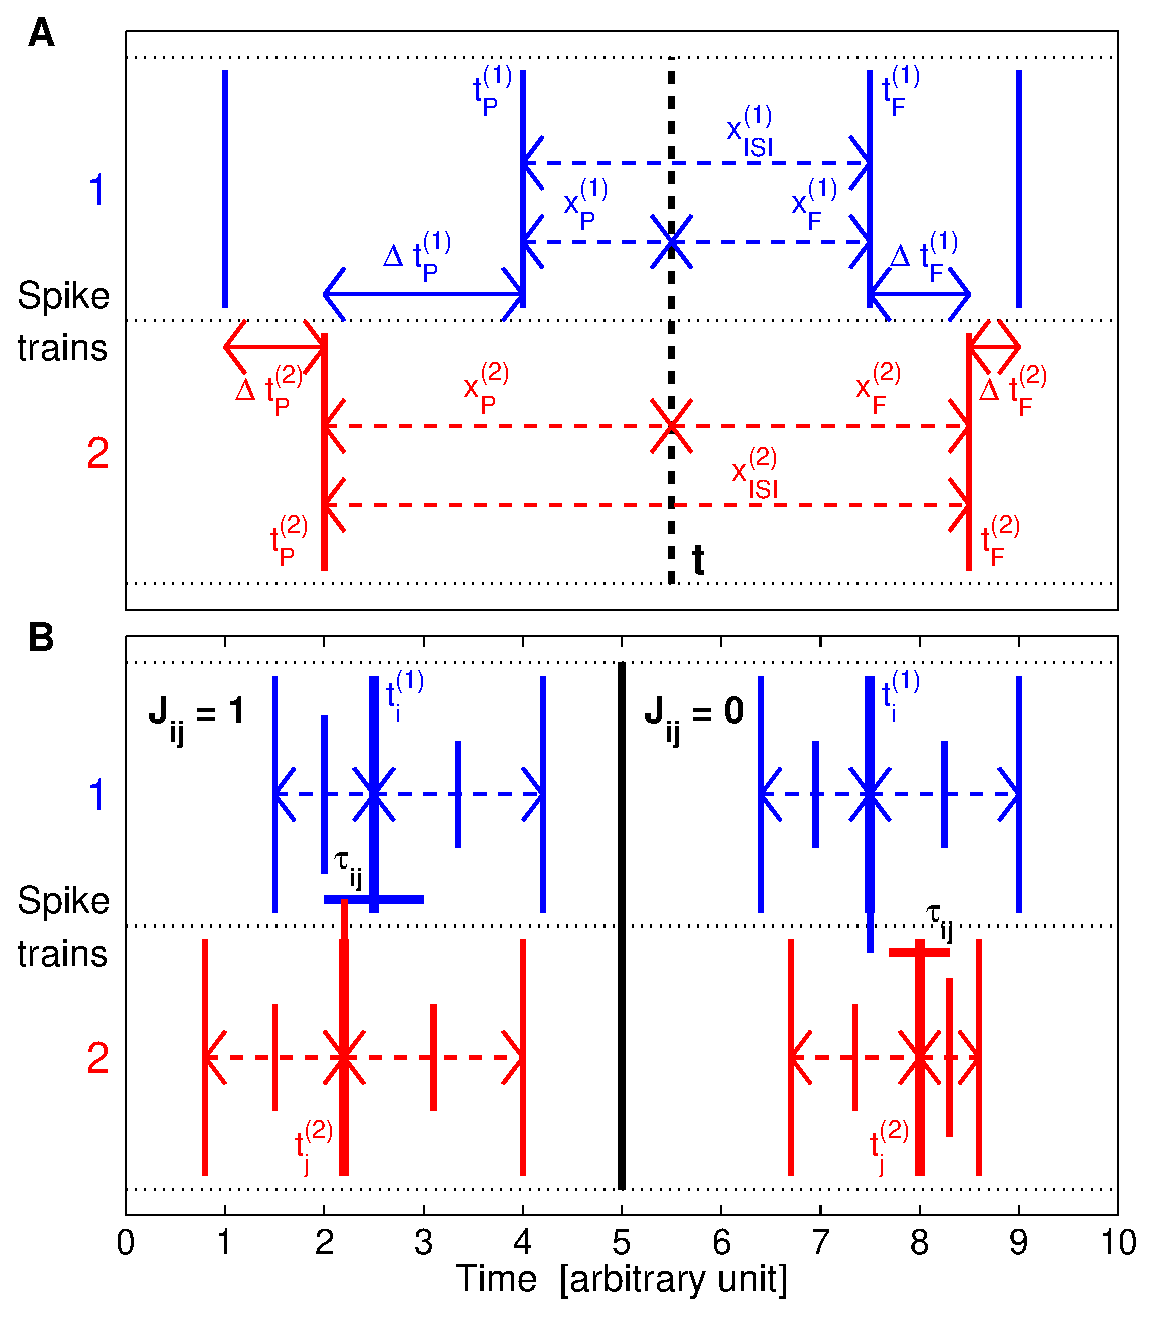
\includegraphics[width=85mm]{ISI_SPIKE_ES_ILLU.eps}
    \caption{\abb\label{fig:ISI-SPIKE-ES-Illustration} A.  ISI- and SPIKE-distance. Illustration of the local quantities needed to define the dissimilarity profiles $I (t)$ and $S (t)$ for an arbitrary time instant $t$.    B. Event synchronization. Illustration of the first variant with adaptive coincidence window. While the middle spikes in the first half are coincident, the middle spikes in the second half are not.}
\end{figure}
%
% #########################################################################################
% #########################################################################################
% ################################## Figure: ISI-SPIKE-ES-Illustration ###########################
% #########################################################################################
% #########################################################################################

The dissimilarity profile is calculated in two steps: First for each spike the distance to the nearest spike in the other spike train is calculated, then for each time instant the relevant spike time differences are selected, weighted, and normalized. Here `relevant' means local; each time instant is surrounded by four corner spikes: the preceding spike from the first spike train $t_{\mathrm {P}}^{(1)}$, the following spike from the first spike train $t_{\mathrm {F}}^{(1)}$, the preceding spike from the second spike train $t_{\mathrm {P}}^{(2)}$, and, finally, the following spike from the second spike train $t_{\mathrm {F}}^{(2)}$. Each of these corner spikes can be identified with a spike time difference, for example, for the previous spike of the first spike train
%
\begin{equation} \label{eq:Delta-Corner-Spike}
     \Delta t_{\mathrm {P}}^{(1)} (t) = \min_i (| t_{\mathrm {P}}^{(1)} (t) - t_i^{(2)} |)
\end{equation}
%
and analogously for $t_{\mathrm {F}}^{(1)}$, $t_{\mathrm {P}}^{(2)}$, and $t_{\mathrm {F}}^{(2)}$  (see Fig. \ref{fig:ISI-SPIKE-ES-Illustration}). For each spike train separately a locally weighted average is employed such that the differences for the closer spike dominate; the weighting factors depend on
%
\begin{equation} \label{eq:Prev-Spike-Dist}
     x_{\mathrm {P}}^{(n)} (t) = t - t_{\mathrm {P}}^{(n)} (t)
\end{equation}
%
and
%
\begin{equation} \label{eq:Foll-Spike-Dist}
     x_{\mathrm {F}}^{(n)} (t) = t_{\mathrm {F}}^{(n)} (t) - t,
\end{equation}
%
the intervals to the previous and the following spikes for each neuron $n = 1, 2$. The local weighting for the spike time differences of the first spike train reads
%
\begin{equation} \label{eq:Bi-Spike-Diss-First}
     S_1 (t) = \frac{\Delta t_{\mathrm {P}}^{(1)} (t) x_{\mathrm {F}}^{(1)} (t) + \Delta t_{\mathrm {F}}^{(1)} (t) x_{\mathrm {P}}^{(1)} (t)}{x_{\mathrm {ISI}}^{(1)} (t)}
\end{equation}
%
and analogously $S_2 (t)$ is obtained for the second spike train. Averaging over the two spike train contributions and normalizing by the mean interspike interval yields
%
\begin{equation} \label{eq:Bi-Spike-Diss-Intermediate}
     S'' (t) = \frac{S_1 (t) + S_2 (t)}{2 \langle x_{\mathrm {ISI}}^{(n)} (t) \rangle_n}.
\end{equation}

This quantity weights the spike time differences for each spike train according to the relative distance of the corner spike from the time instant under investigation. This way relative distances within each spike train are taken care of, while relative distances between spike trains are not. In order to get these ratios straight and to account for differences in firing rate, in a last step the two contributions from the two spike trains are locally weighted by their instantaneous interspike intervals. This leads to the definition of the dissimilarity profile
%
\begin{equation} \label{eq:Bi-Spike-Diss-Improved}
     S (t) = \frac{S_1 (t) x_{\mathrm {ISI}}^{(2)} (t) + S_2 (t) x_{\mathrm {ISI}}^{(1)} (t)}{2 \langle x_{\mathrm {ISI}}^{(n)} (t) \rangle_n^2}.
\end{equation}
%
Since the dissimilarity profile $S (t)$ is obtained from a linear interpolation of piecewise constant quantities, it is piecewise linear (with potential discontinuities at the spikes). This dissimilarity profile and the SPIKE-distance $D_S$ as its average are both bounded in the interval $[0, 1]$. The distance value $D_S = 0$ is obtained for identical spike trains only.



\subsubsection{\label{sss:Realtime-Spike-Distance} Realtime SPIKE-distance}

The realtime SPIKE-distance $D_{S_r}$ is a modification of the SPIKE-distance with the key difference that the corresponding time profile $S_r(t)$ can be calculated online because it relies on past information only \footnote{For the ISI-distance no such causal realtime extension is possible, since it relies on the instantaneous ISI-values and thus requires knowledge about the following spikes. Similarly, there is no future ISI-distance either.}. From the perspective of an online measure, the information provided by the following spikes, both their position and the length of the interspike interval, is not yet available. Like the regular (improved) SPIKE-distance $D_S$, this causal variant is also based on local spike time differences but now only two corner spikes are available, and the spikes of comparison are restricted to past spikes, e.g., for the preceding spike of the first spike train
%
\begin{equation} \label{eq:Delta-Corner-Spike-Realtime}
     \Delta t_{\mathrm {P}}^{(1)} (t) = \min_i (| t_{\mathrm {P}}^{(1)} (t) - t_i^{(2)} |), t_i \leq t.
\end{equation}
%
Since there are no following spikes available, there is no local weighting, and since there is no interspike interval, the normalization is achieved by dividing the average corner spike difference by twice the average time interval to the preceding spikes (Eq. \ref{eq:Prev-Spike-Dist}). This yields a causal indicator of local spike train dissimilarity:
%
\begin{equation} \label{eq:Bi-Spike-Diss-RT}
    S_r (t) = \frac{ \Delta t_{\mathrm {P}}^{(1)} (t) + \Delta t_{\mathrm {P}}^{(2)} (t)} {4 \langle x_{\mathrm {P}}^{(n)} (t) \rangle_n}.
\end{equation}


\subsubsection{\label{sss:Future-Spike-Distance} Future SPIKE-distance}

The future SPIKE-distance $D_{S_f}$ can be used in triggered temporal averaging in order to evaluate the effect of certain spikes or of certain stimuli features on future spiking. It is the inverse measure to the realtime SPIKE-distance but instead of relying on past information only it relies on future information only. Again for each time instant there are just two corner spikes and the potential nearest spikes in the other spike train are future spikes only. Thus the spike time difference for the following spike of the first spike train reads
%
\begin{equation} \label{eq:Delta-Corner-Spike-Future}
     \Delta t_{\mathrm {F}}^{(1)} (t) = \min_i (| t_{\mathrm {F}}^{(1)} (t) - t_i^{(2)} |), t_i > t,
\end{equation}
%
and accordingly for the following spike of the second spike train. In analogy to Eq. \ref{eq:Bi-Spike-Diss-RT}, an indicator of local spike train dissimilarity is obtained as follows:
%
\begin{equation} \label{eq:Bi-Spike-Diss-FT}
    S_f (t) = \frac{ \Delta t_{\mathrm {F}}^{(1)} (t) + \Delta t_{\mathrm {F}}^{(2)} (t)} {4 \langle x_{\mathrm {F}}^{(n)} (t) \rangle_n}.
\end{equation}	



\subsection{\label{ss:Improvements} Improvements in this implementation}

\subsubsection{\label{sss:Edge-effect} Correction of the edge effect for the SPIKE-distance}

In previous versions of the SPIKE-distance the ambiguity regarding the definition of the initial (final) distance to the preceding (following) spike as well as the very first and the very last interspike intervals was resolved by adding to each spike train an auxiliary leading spike at time $t = 0$ and an auxiliary trailing spike at time $t = T$. This lead to spurious synchrony at the edges where by construction the dissimilarity profile reached the zero value. Here we follow a suggestion by Conor Houghton (personal communication) and at least partly correct this edge effect. We describe the correction for the beginning of the recording, it is an analogous mirror image at the end of the recording.

We count the auxiliary spikes as normal spikes which can be nearest neighbor to other spikes. But instead of calculating their spike time distance (which is always zero) we use the spike time difference of the first real spike. For the first interspike interval we know that it is at least the distance to the first spike $t_1-t_0 = t_1$ but it could be longer. So to take the local firing rate (or its inverse) into consideration we set
%
\begin{equation} \label{eq:Corrected-First-ISI}
    x_{\mathrm {ISI}} (0) = \max ( t_1, t_2 - t_1 ).
\end{equation}
%
where we use the length of the first known interspike interval $t_2-t_1$ as an upper limit of the inverse firing rate. This way we get at least a crude estimate of how much longer the first interspike interval could be.


\subsubsection{\label{sss:Sampling} Increase of memory efficiency by avoiding oversampling}

Earlier versions of the codes for calculating event synchronization and the ISI- and the SPIKE-distance relied on equidistantly sampled dissimilarity profiles. Typically the precision was set to the sampling interval of the neuronal recording. Since the dissimilarity profile has to be calculated and stored for each pair of spike trains, this resulted, for each measure, in a matrix of order `number of sampled time instants' $\times$ `number of spike train pairs' (i.e., $\# (t_s) \times N(N-1)/2$). For small sampling intervals and a large number of recorded spike trains this lead to memory problems.

In SPIKY we use an optimized and more memory-efficient way of storing the data where we make use of the fact that the dissimilarity profiles $I (t)$ of the ISI-distance is piecewise constant and the dissimilarity profile $S (t)$ of the SPIKE-distance is piecewise linear with each interval running from one spike of the pooled spike train to the next one. Thus for each such interval (and for each pair of spike trains) we have to store only one value for the ISI-distance and two values for the SPIKE-distance, one at the beginning and one at the end of the interval (see Figure \ref{fig:No-sampling}). Typically the storage space required will be much smaller than for dissimilarity profiles sampled with a reasonable precision. This new implementation is not only far more memory-efficient, it is also slightly faster (cf. Section \ref{ss:Comparison}) and in particular it computes the exact distance values without any (spurious) dependence on the sampling interval.
%
% #########################################################################################
% #########################################################################################
% ############################################# Figure: No sampling #######################
% #########################################################################################
% #########################################################################################
%
\begin{figure}
    \includegraphics[width=85mm]{No_sampling.eps}
    \caption{\abb\label{fig:No-sampling} Illustration of the memory efficient storage of the dissimilarity profile for both the ISI- and the SPIKE-distance.}
\end{figure}
%
% #########################################################################################
% #########################################################################################
% ############################################# Figure: No sampling #######################
% #########################################################################################
% #########################################################################################

For the dissimilarity profiles of both the ISI- and the SPIKE-distance there are instantaneous jumps at the times of the spikes since this is where the lengths of the interspike intervals and the identity of the previous and the following spikes change abruptly. In contrast to the calculation based on sampling we get the exact result since each spike is both the previous and the next spike and there is no need anymore to `cut the corners' of the dissimilarity profiles as had to be done for the sampled dissimilarity profiles. The dissimilarity profiles $S_r(t)$ and $S_f (t)$ of the real-time and the future SPIKE-distances are hyperbolic but for these measures the exact result can be obtained by piecewise integration over all intervals of the pooled spike train. While we use these integration schemes to calculate the exact values, for the time-resolved visualization we use linear interpolations within the individual intervals in order to reach the same low computational complexity that we obtain for the regular SPIKE-distance.



\subsection{\label{ss:Event-Synchronization} Event synchronization}

Event synchronization (\citeauthor{QuianQuiroga02b}, \citeyear{QuianQuiroga02b}; cf. \citeauthor{Kreuz07c}, \citeyear{Kreuz07c} and \citeauthor{Kreuz11b}, \citeyear{Kreuz11b}) works as a coincidence detector quantifying the level of synchrony from the number of quasi-simultaneous appearances of spikes. There are two variants. The main variant is parameter- and scale-free, since the time lag $\tau_{ij}$ up to which two spikes $t_i^{(1)}$ and $t_j^{(2)}$ are considered to be synchronous is adapted to the local spike rates (see Fig. \ref{fig:ISI-SPIKE-ES-Illustration}B):
%
\begin{equation} \label{eq:Event-MaxDist}
    \tau_{ij} = \min \{t_{i+1}^{(1)} - t_i^{(1)}, t_i^{(1)} - t_{i-1}^{(1)},
                           t_{j+1}^{(2)} - t_j^{(2)}, t_j^{(2)} - t_{j-1}^{(2)}\}/2.
\end{equation}
%
In contrast, the second variant uses a fixed coincidence window $\tau$.

The function $c(1|2)$ counts the appearances of a spike in the first spike train shortly after a spike in the second spike train:
%
\begin{equation} \label{eq:Event-Count}
    c (1|2) = \sum_{i=1}^{M_1} \sum_{j=1}^{M_2} J_{ij},
\end{equation}
%
where
%
\begin{equation} \label{eq:Event-Synchronicity}
    J_{ij} = \begin{cases}
                      1     & {\rm if} ~~ 0 < t_i^{(1)} - t_j^{(2)} \leq \tau_{ij} \cr
                      1/2   & {\rm if} ~~ t^{(1)}_i = t^{(2)}_j \cr
                      0     & {\rm otherwise}.
                  \end{cases}
\end{equation}
%
Here we used the definition of the first (scale-free) variant, for the second variant just replace $\tau_{ij}$ with $\tau$. Then with $c(2|1)$ defined accordingly, event synchronization can be written as
%
\begin{equation} \label{eq:Event-Synchro}
    Q = \frac {c (2|1) + c (1|2)} {\sqrt{M_1 M_2}}.
\end{equation}
%
In order to get a time-resolved measure of event synchronization, we calculate the local `derivative' of the $Q$-function
%
\begin{equation} \label{eq:Window-Event-Synchro}
    E = \frac {Q (n+\Delta n) - Q (n-\Delta n)} {\sqrt{\Delta n_1 \Delta n_2}}.
\end{equation}
%
where $\Delta n_1$ and $\Delta n_2$ are the numbers of events in the interval $[n-\Delta n, n+\Delta n]$ with $n$ here referring to the number of intervals in the pooled spike train.

Unfortunately, $E$ is not any longer parameter-free. The time resolution is governed by the window size $\Delta n$. For the second variant of event synchronization the fixed coincidence window $\tau$ constitutes a second parameter.

A suitably normalized distance is obtained by inversion $D_E=E-1$, with $D_E = 0$ if and only if all spikes within the window coincide (or if there are no spikes at all). XXXXX Orientation in figures? XXXXX

In the SPIKY-framework the overall value within a certain time interval is obtained as the temporal average of the dissimilarity profile over this interval. While this is the actual definition of the ISI- and the SPIKE-distance this (cf. Eq. \ref{eq:Temporal-Average}), for event synchronization it is more complicated since there the temporal profile has been obtained as the derivative of the cumulative function $Q$. XXXXXXXXXXXX

This is not necessarily identical to the regular event synchronization obtained from the cumulative function $Q$\ref{eq:Event-Synchro}. But numerical analysis reveals that the deviation is typically less than XXXXX.

Fig. \ref{fig:PSTH-ES} shows a comparison between the Peri-Stimulus Time Histogram and event synchronization. It shows that the PSTH, in contrast to event synchronization, is not a measure of spike train synchrony (see also \citeauthor{Kreuz11}, \citeyear{Kreuz11}). Since it is invariant to shuffling spikes among the spike trains yields the same value regardless of how spikes are distributed among the different spike trains.

stress: often optimization of parameters needed

not yet finished XXXXX

%
% #########################################################################################
% #########################################################################################
% ###################################### Figure: PSTH & ES ################################
% #########################################################################################
% #########################################################################################
%
\begin{figure}
    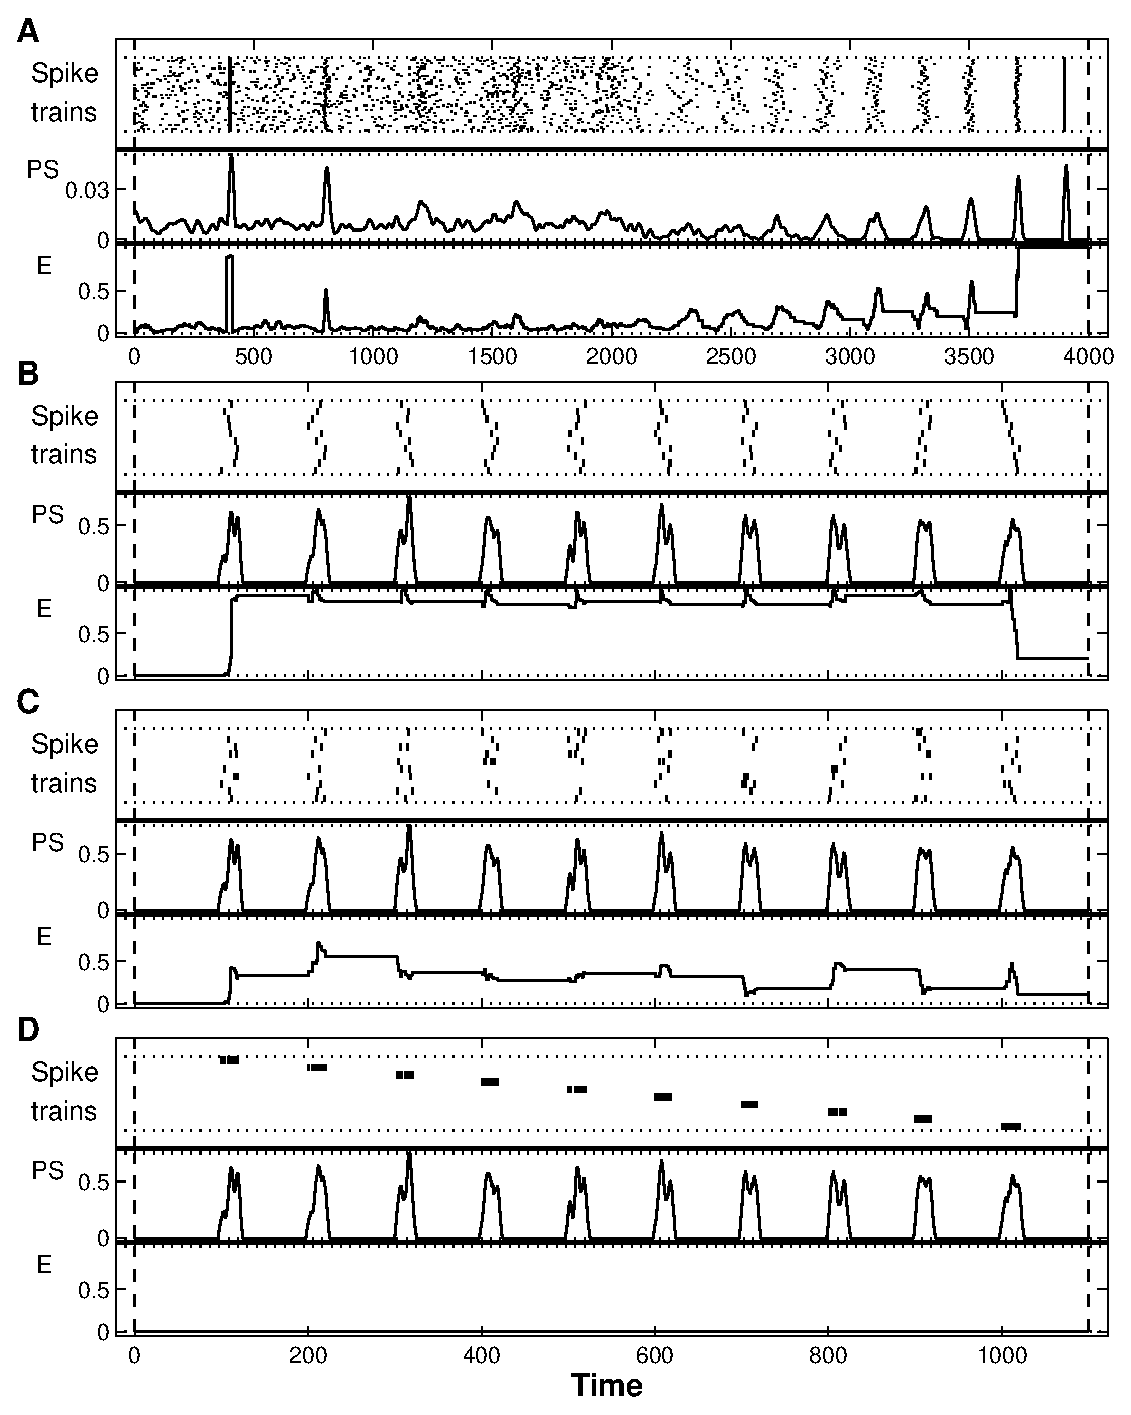
\includegraphics[width=85mm]{PSTH_ES.eps}
    \caption{\abb\label{fig:PSTH-ES} Comparison of PSTH and event synchronization. A. multivariate example with $50$
spike trains. In the first half within the noisy background there are $4$ regularly spaced spiking events with increasing jitter. The second half consists of $10$ spiking events with decreasing jitter but now without any noisy background. PSTH and event synchronization exhibit very similar profiles. The dissimilarity profile of the SPIKE-distance for the same example can be found in Fig. 2B of \citet{Kreuz13}.    B-D. By construction the pooled spike train of these examples is identical consisting of $10$ evenly spaced bursts. The only difference is the distribution of the spikes among the individual spike trains. B. High reliability. C. Random distribution of spikes among spike trains. D. Synfire chain. Whereas the PSTH is identical, event synchronization correctly transitions from high to intermediate and low synchrony.}
\end{figure}
%
% #########################################################################################
% #########################################################################################
% ###################################### Figure: PSTH & ES ################################
% #########################################################################################
% #########################################################################################
%
	
% *************************************************************************************
% *************************************************************************************
% ********************************** Section: Information reduction *******************
% *************************************************************************************
% *************************************************************************************
%

\section{\label{s:Information-reduction} Levels of information reduction}

The ISI- and the SPIKE-distance combine a variety of properties that make them well suited for applications to real data. In particular, they are conceptually simple, computationally efficient, and easy to visualize in a time-resolved manner. By taking into account only the preceding and the following spike in each spike train, these distances rely on local information only. They are also time-scale-adaptive since the information used is not contained within a window of fixed size but rather within a time frame whose size depends on the local rate of each spike train.

Moreover, the sensitivity to spike timing and the instantaneous reliability achieved by the SPIKE-distance opens up many new possibilities in multi-neuron spike train analysis \citep{Kreuz13}. These build upon the fact that there are several levels of information reduction all of which we describe in the following. As illustration we use the detailed analysis of an artificially generated spike train dataset (see upper subplot of Fig. \ref{fig:SPIKE-Representations}A for the rasterplot). 
%
% #########################################################################################
% #########################################################################################
% ##################################### Figure: Representations ###########################
% #########################################################################################
% #########################################################################################
%
\begin{figure}
    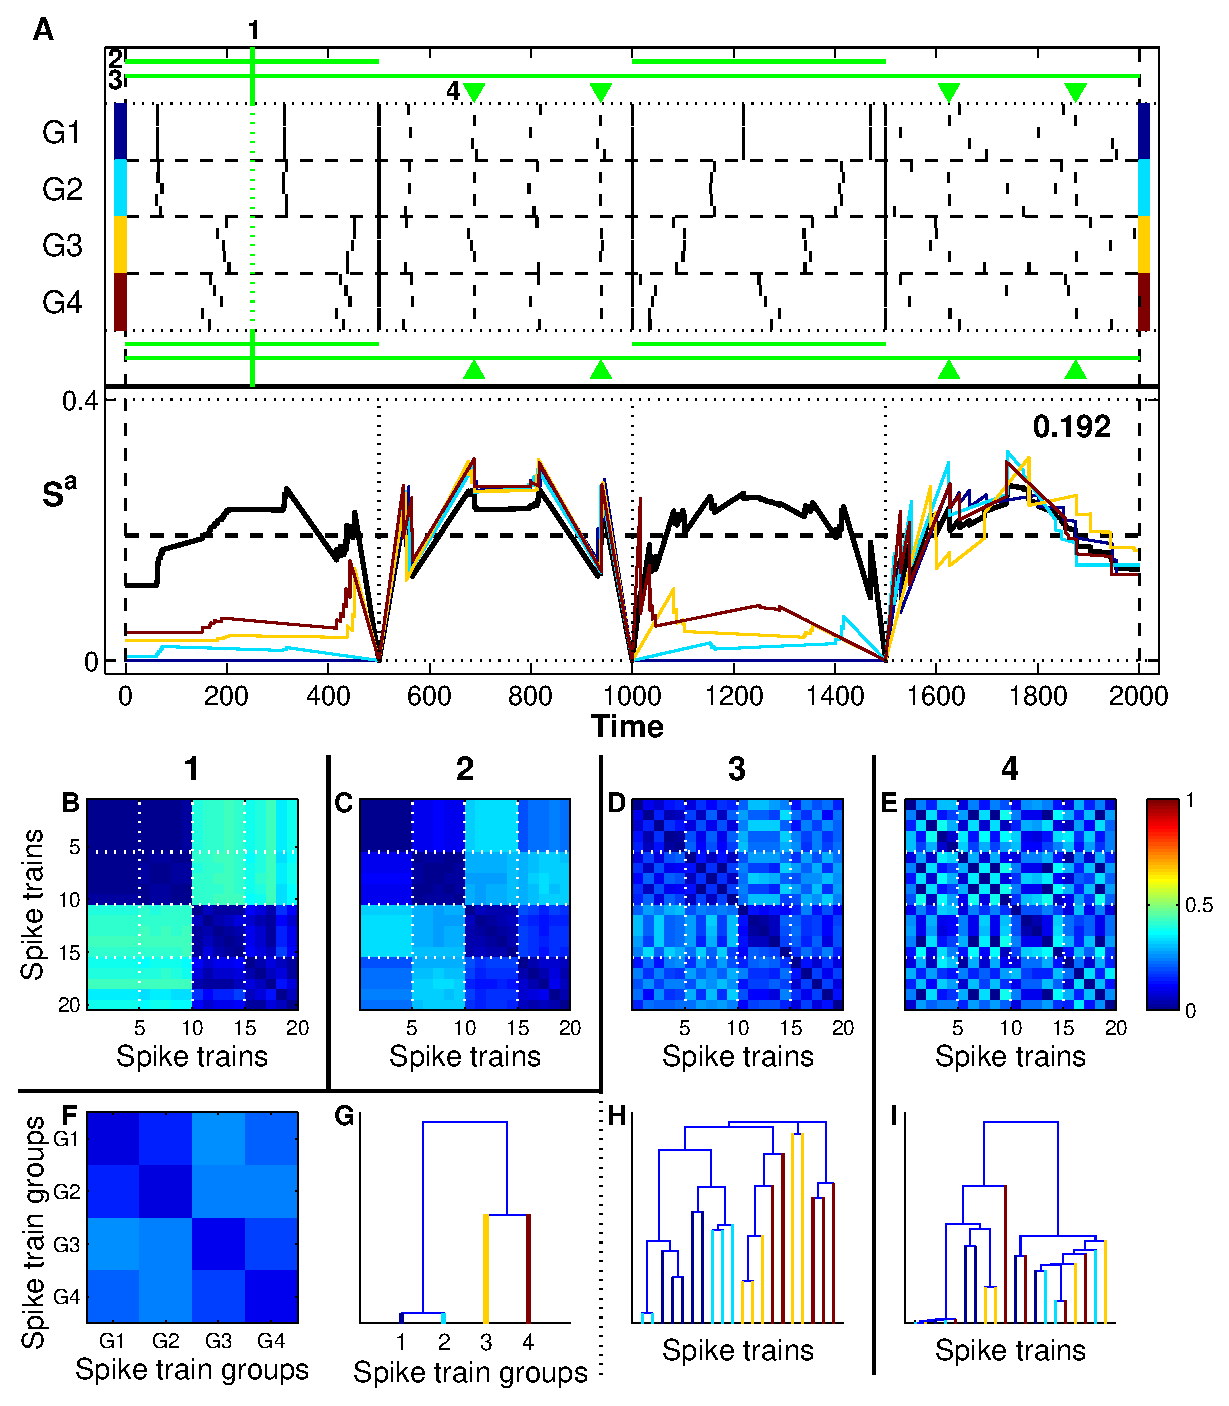
\includegraphics[width=85mm]{SPIKE_Representations.eps}
    \caption{\abb\label{fig:SPIKE-Representations} The different levels of information reduction for the SPIKE-distance.  A. Top: Spike rasterplot of $20$ artificially generated spike trains divided in $4$ spike train groups of $5$ spike trains each. The clustering behavior changes every $500$ ms. Bottom: Dissimilarity profiles of the SPIKE-distance for the four spike train groups (thin color-coded lines) and for all spike trains (thick black line). The overall dissimilarity is defined as the temporal average of the dissimilarity profile of all spike trains ($0.192$ in this case) and is marked by a black horizontal line.  B-E. Matrices of pairwise instantaneous dissimilarity values for a single time instant, for two selective averages and for a triggered average.  F. Matrices of overall pairwise instantaneous dissimilarity values for the $4$ spike train groups.  G. Dendrogram of spike train group matrix in F.  H-I. Dendrogram of spike train matrices in D and E. Note that the triggered averages in contrast to the overall average captures the local similarity between $5$ of the spike trains.}
\end{figure}
%
% #########################################################################################
% #########################################################################################
% ##################################### Figure: Representations ###########################
% #########################################################################################
% #########################################################################################

\subsection{\label{ss:Full-matrix-and-cross-sections} Full matrix and cross sections}

The starting point is the most detailed representation in which one instantaneous value is obtained for each pair of spike trains (see Eq. \ref{eq:Bi-Spike-Diss-Improved}). This representation could be viewed as a movie of a symmetric pairwise dissimilarity matrix in which each frame corresponds to one time instant (an example can be found in the supplementary material of \citep{Kreuz13}). For a movie of finite length the time axis necessarily has to be sampled but in principle this most detailed representation is continuous and consists of an infinite number of values. However, since all dissimilarity profiles are piecewise linear (with potential discontinuities only at the times of the spikes) there is a lot of redundancy. Using the most compact and memory-efficient representation one can store all pairwise dissimilarity profiles in a matrix of size `number of interspike intervals in the pooled spike train' $\times$ `number of spike train pairs' ($\times 2$ for the SPIKE-distance, see Section \ref{sss:Sampling}).

From this matrix, it is possible to extract any desired information. By selecting a pair of spike trains, one obtains the bivariate dissimilarity profile $S (t)$ for this pair of spike trains. Selecting a time instant $t_s$ (and using linear interpolation for time instants in between spikes) yields an instantaneous matrix of pairwise spike train dissimilarities $S_{mn}(t_s)$ (see Fig. \ref{fig:SPIKE-Representations}B). This matrix can be used to divide the spike trains into instantaneous clusters, that is, groups of spike trains with low intra-group and high inter-group dissimilarity.

\subsection{\label{ss:Spatial-and-temporal-Averaging} Spatial and temporal averaging}

Another way to reduce the information of the dissimilarity matrix is averaging. There are two possibilities that commute: the spatial average over spike train pairs and the temporal average. Since the spatial average over spike train pairs can be done locally it yields a dissimilarity profile for the whole population. Examples for averages over four different spike train groups as well as over all spike trains are shown in the lower subplot of Fig. \ref{fig:SPIKE-Representations}A. Temporal averaging over certain intervals on the other hand leads to a bivariate distance matrix (see Fig. \ref{fig:SPIKE-Representations}C and D for examples of non-continuous and continuous intervals). In real data, these temporal intervals could be chosen to correspond to different external conditions such as normal vs. pathological, asleep vs. awake, target vs. non-target stimulus, or presence/absence of a certain channel blocker. 

A combination of temporal and spatial averaging can be seen in Fig. \ref{fig:SPIKE-Representations}F. This dissimilarity matrix is obtained from the overall temporal average shown in Fig. \ref{fig:SPIKE-Representations}D by (spatially) averaging over the $16$ submatrices and thus depicts the pairwise spike train group dissimilarity ($4 \times 4$ instead of $20 \times 20$). Fig. \ref{fig:SPIKE-Representations}G shows the respective dendrogram. In applications to real data, these groups could be different neuronal populations or responses to different stimuli, depending on whether the spike trains were recorded simultaneously or successively. Finally, successive application of the spatial average over all spike train pairs and the temporal average over the whole interval results in just one single distance value that describes the overall level of synchrony for the whole dataset. In Fig. \ref{fig:SPIKE-Representations}A this value is stated in the upper right of the lower subplot.


\subsection{\label{ss:Triggered-Averaging} Triggered averaging}

The fact that there are no limits to the temporal resolution allows further analyses such as internally or externally triggered temporal averaging. Here, the matrices are averaged over certain trigger time instants only. The idea is to check whether this triggered temporal average is significantly different from the global average since this would indicate that something peculiar is happening at these trigger instants. The trigger times can either be obtained from external influences (such as the occurrence of certain features in a stimulus) or from internal conditions (such as the spike times of a certain spike train). External triggering is a standard tool to address questions of neural coding, for example, it can be used to evaluate the influence of localized stimulus features on the reliability of neurons under repeated stimulation. In multi-neuron data, internal triggering might help to uncover the connectivity in neural networks or to detect converging or diverging patterns of firing propagation. An example is shown in Fig. \ref{fig:SPIKE-Representations}E. Here, neurons $2$, $9$, $14$, and $19$ follow the $7$-th neuron during the 2nd and the 4th $500$-ms subinterval. This can be revealed by triggering on the spike times of neuron $7$ during these subintervals. The difference between the triggered dissimilarity matrix of \ref{fig:SPIKE-Representations}E and the dissimilarity matrix of the full interval in Fig. \ref{fig:SPIKE-Representations}E can be seen best by comparing the respective dendrograms in Fig. \ref{fig:SPIKE-Representations}H and I.

%
% *************************************************************************************
% *************************************************************************************
% ************************************* Section: SPIKY ********************************
% *************************************************************************************
% *************************************************************************************
%
\section{\label{s:SPIKY} SPIKY}

SPIKY is a graphical user interface for monitoring synchrony between artificially simulated or experimentally recorded neuronal spike trains. It contains implementations of the ISI- and the SPIKE-distance (including simulations of its realtime and future variants) as well as event synchronization which allow interactive access to all the different representations described in Section \ref{s:Information-reduction}. All source codes are written in Matlab (MathWorks Inc, Natick, MA, USA) with the most time-consuming loops coded in MEX-files \footnote{In our case these are subroutines written in C. However, as some users may not have access to a suitable C compiler, SPIKY contains the (slower) pure Matlab code as well.}. SPIKY is not stand-alone but requires Matlab to run.


\subsection{\label{ss:Access} Access to SPIKY and how to get started}

SPIKY is distributed under a BSD licence (Copyright (c) 2014, Thomas Kreuz, Nebojsa Bozanic. All rights reserved.). A zip-package containing all the necessary files can be accessed for free on the \href{http://www.fi.isc.cnr.it/users/thomas.kreuz/Source-Code/SPIKY.html}{download page} (\url{http://www.fi.isc.cnr.it/users/thomas.kreuz/Source-Code/SPIKY.html}). This package also contains a folder with lots of documentation (such as a FAQ-file and an introduction to all individual elements and all individual files of SPIKY). Further information and many demonstrations (both images and movies) can be found on the download page and on the \href{https://www.facebook.com/SPIKYgui}{SPIKY Facebook-page} (\url{https://www.facebook.com/SPIKYgui}). Both of these pages are used to announce updates and distribute the latest information about new features. They also provide the user with an opportunity to provide feedback and ask questions.

The Facebook-page includes various screen recordings with voice-over in which the user is guided step by step through some of the most important features of SPIKY. All of these movies can also be viewed on the \href{https://www.youtube.com/channel/UCgSz0YQ5lWdVF0_Z1FNN0Bw}{SPIKY Youtube-channel} (\url{https://www.youtube.com/channel/UCgSz0YQ5lWdVF0_Z1FNN0Bw}).

After having downloaded SPIKY from the download page the user has to first extract the zip-package which leaves all files in one folder named `SPIKY'. If the system has a suitable MEX-compiler installed, the MEX-files can be compiled from within this folder by running the m-file `SPIKY\_compile\_MEX'. The last step is to run the m-file `SPIKY'.

When SPIKY is running, the user can find quick information about the individual elements of the graphical user interface by activating the `Hints'-checkbox in the `Options'-Menu. Hovering with the mouse cursor above the elements of interest will then show short hints. An overview of all the information contained in the hints can be found in the documentation file `SPIKY-Elements.doc'. Furthermore, at each step the suggested element for the next user action is highlighted by a bold font. 

To get the user started quickly, SPIKY provides a few (artificial) example datasets from previous publications. The most useful example is the entry `Clustering' in the `Selection: Data'-listbox. This dataset has already been used in several figures as well as in the supplementary movie of \cite{Kreuz13}. A good introduction to SPIKY would be to follow this example through till the end advancing from panel to panel by pressing the highlighted button. In a second step one could reset and run the same example again while changing some parameters in order to see the consequences. Note that it is not necessary to set all the parameters each time when SPIKY is started. Rather it is possible to use the file `SPIKY\_f\_user\_interface' to set and modify the spike train data as well as the parameters (again refer to the dataset `Clustering' for an example).


\subsection{\label{ss:Structure} Structure and workflow of SPIKY}

Overall, SPIKY has a rather linear workflow, however, it is much more interactive than previous implementations of the measures and there are many potential shortcuts and loops along the way. As you can see in the SPIKY-flowchart in Fig. \ref{fig:SPIKY-Flowchart}, the general flow is clearly directed from the input of spike train data to the output of results. So the first step the user has to do is to give SPIKY spike train data (i.e. sequences of spike times) to work with. There are three possibilities to do so: one can make use of predefined examples, load data from a file, or employ the spike train generator (see Section \ref{sss:Input} for more details).
%
% #########################################################################################
% #########################################################################################
% ########################################### Figure: Flowchart ###########################
% #########################################################################################
% #########################################################################################
%
\begin{figure}
    \includegraphics[width=85mm]{SPIKY_Flowchart.eps}
    \caption{\abb\label{fig:SPIKY-Flowchart} Flowchart describing the workflow of SPIKY from 	the input of spike train data to the output of results. A typical SPIKY-session begins at the top with `Get data', then goes clockwise and ends on the left with `Get results'. In the center of the circle the SPIKY-logo is depicted.}
\end{figure}
%
% #########################################################################################
% #########################################################################################
% ########################################### Figure: Flowchart ###########################
% #########################################################################################
% #########################################################################################

Once the full dataset is there, modification is still possible. One can restrict the analysis to a specific subset, e.g., select a smaller time window and/or a subset of spike trains. It is also possible to impose some external structure on the rasterplot (spike trains vs time). SPIKY allows the definition of two types of time markers (e.g. specific events such as seizure onset and offset in epilepsy, trigger onset during stimulation etc.) and two types of spike train separators (e.g. neurons from the left vs. neurons from the right hemisphere). It also enables the user to define spike train groups. Depending on the setup these could be spike trains recorded in different brain regions or upon presentation of different kinds of stimuli. Fig. \ref{fig:Movie-Screenshot} shows an example of a raster plot with annotations marking all these different elements.
%
% #########################################################################################
% #########################################################################################
% #################################### Figure: Movie-Screenshot ###########################
% #########################################################################################
% #########################################################################################
%
\begin{figure}
    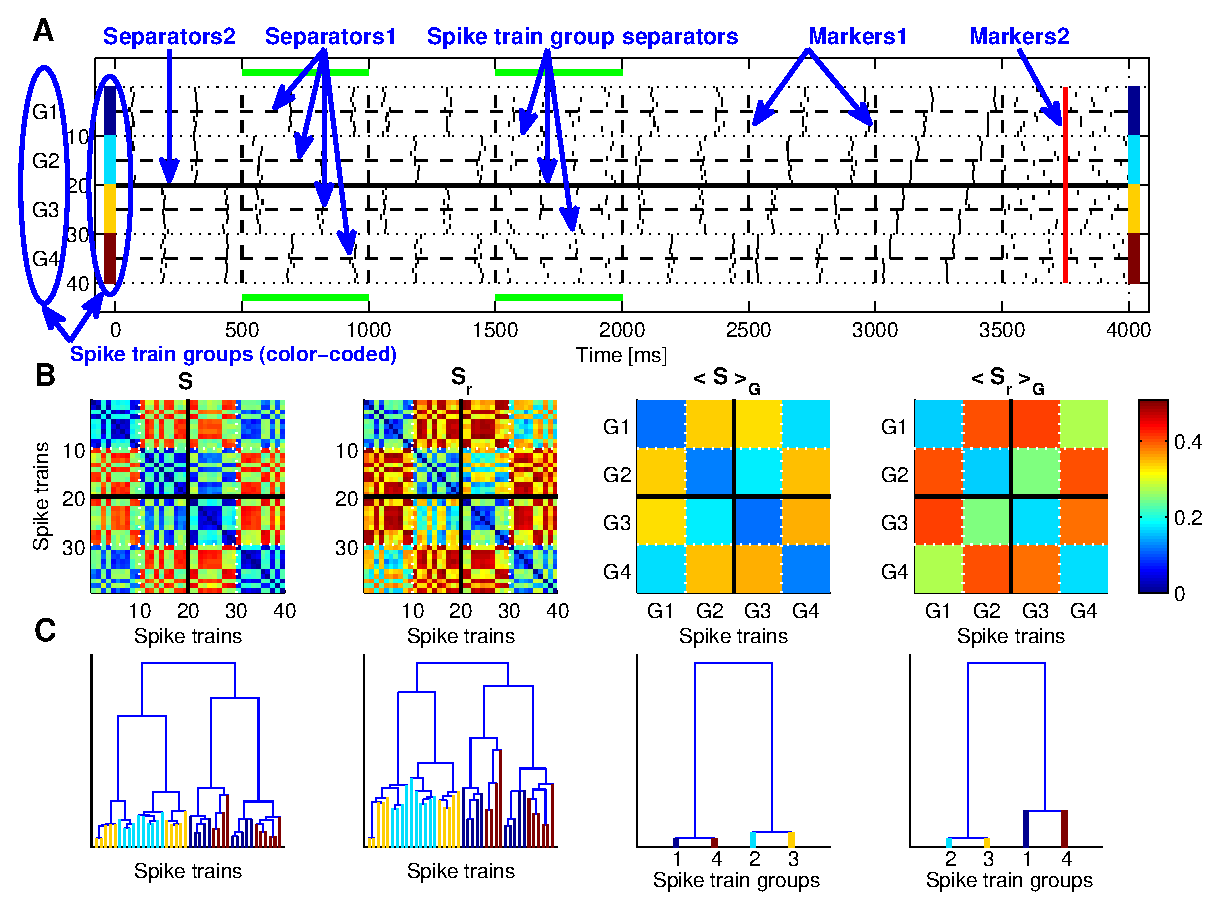
\includegraphics[width=85mm]{Movie_Screenshot.eps}
    \caption{\abb\label{fig:Movie-Screenshot} Annotated screenshot from a movie.   A. Artificially generated spike trains.   B. Dissimilarity matrices obtained by averaging over two separate time intervals for both the regular and the real-time SPIKE-distance as well as their averages over subgroups of spike trains (denoted by $<\cdot>_G$).   C. Corresponding dendrograms.}
\end{figure}
%
% #########################################################################################
% #########################################################################################
% #################################### Figure: Movie-Screenshot ###########################
% #########################################################################################
% #########################################################################################

After updating all of these data parameters the next step is to select the measures to be calculated. In addition to the measures described in the Appendix \ref{s:Measures} we also include the Peri-Stimulus Time Histogram as a time-resolved standard approach widely used in spike train analysis. However, note that the PSTH is a complementary approach which describes overall firing rate and (to some precision) timing. It is not a measure of spike train synchrony \citep{Kreuz11} since it is invariant to shuffling spikes among the spike trains yielding the same value regardless of how spikes are distributed among the different spike trains (see Fig. \ref{fig:PSTH-ES}). At the same time the user can select successive frames for a temporal analysis of spike train patterns. These can be individual time instants for cross sections, temporal intervals for selective averages and sequences of time instants for triggered averages (see Section \ref{s:Information-reduction}).

Now the actual calculation of the measures takes place. For reasonably sized datasets this should take at most a few seconds. Larger datasets are divided in smaller subintervals and the calculation will be performed in a loop which might take longer (cf. Section \ref{ss:Limitations}). It is at this point that SPIKY becomes truly interactive. Now the user can switch between different representations of the results (such as dissimilarity profiles, dissimilarity matrices and dendrograms). Regarding matrices and dendrograms one can decide whether one wants to compare different representations or look at them in sequence.

The presentation can be restricted to smaller time windows and/or subsets of spike train, and temporal and spatial averaging (for example moving average and average over spike train groups) can be performed. It is possible to add further figure elements such as spike number histograms, overall averages, or dissimilarity profiles for individual spike train groups. At this stage the user can also retrospectively change the appearance of all the individual elements of the figure (see Section \ref{sss:Figure-Layout} for more details). Finally, SPIKY allows to extract both data and results to the Matlab workspace for further analysis, and it is also possible to save individual figures as postscript-file or a sequence of images as an `avi'-movie (for more details see Section \ref{sss:Output}).


\subsubsection{\label{sss:Input} Input}

There are three different possibilities to input spike train data into SPIKY.

The first option is to select one of the predefined examples which are generated using Matlab-code. Initially these are the examples used in \citep{Kreuz13} but one can also define new examples.

The second option is to load spike train data from a file. Two different file formats are allowed, `.mat' and `.txt' (ASCII) files. For the mat-files SPIKY currently allows three different kinds of input formats (further formats can be added on demand).

\begin{itemize}
\item cell arrays (ca) with just the spike times. This is the preferred format used by SPIKY since it is most memory efficient. The two other formats will internally be converted into this format.
\item regular matrices with each row being a spike train and zero padding (zp) in case the spike numbers are different.
\item matrices representing time bins where each zero/one (01) indicates the absence/presence of a spike
\end{itemize}

If case of a mat-file SPIKY looks for a variable called `spikes', if it cannot find it you have the chance to select the variable name (or field name) which contains the spikes via an input mask which provides a hierarchical structure tree of the variable structure. In the text format spike times should be written as a matrix with each row being one spike train. The SPIKY-package contains one example file for all four formats (`testdata\_ca.mat', `testdata\_zp.mat', `testdata\_01.mat' and `testdata.txt').

The third option is to create new spike train data via the spike train generator. After setting some defining variables (number of spike trains, start and end time, sampling interval) you can build your spike trains by using predefined spike train patterns (such as periodic, splay, uniform or Poisson) and/or by manually adding, shifting and deleting individual spikes or groups of spikes.


\subsubsection{\label{sss:Figure-Layout} Figure-Layout}

SPIKY was designed in a way that allows to directly generate figures suitable for publication. To this aim the user is given control over the appearance of every individual element (e.g. fonts, lines etc.) in each type of figure. There are two ways to determine essential properties such as color, font size or line width. Most conveniently, one can use the file `SPIKY\_f\_user\_interface' to define the standard values for all the parameters that describe the principal layout of the figure. But it is also possible to change elements in the active figure while the program is already running. To do so the user has to simply click the right mouse button on the element to be changed. A context menu will appear which lets the user either edit either the properties of individual elements or of all elements of a certain type. This also includes the string property of any font (title, x- and y-labels etc.).

If a figure contains more than one subplot (besides the combined subplot containing the spike rasterplot and dissimilarity profiles these are typically subplots with dissimilarity matrices and dendrograms), it is also possible to change their position and size. To do so just move the cursor to the respective axis (either just left or just below the subplot) and click the right mouse button. Now one can edit all position variables by hand or change the x-position, the y-position, the width and the height individually. In case there are several dissimilarity matrices / dendrograms one can do this either for an individual matrix / dendrogram or for all of them at the same time.


\subsubsection{\label{sss:Output} Output}

From within SPIKY it is possible to extract the spike trains and the results of the analyses (measure profiles, matrices, dendrograms) to the Matlab workspace for further processing. When one clicks the right mouse button on the element whose data one wishes to extract results will be stored in variables such as `SPIKY\_spikes', `SPIKY\_profile\_X\_1', `SPIKY\_profile\_Y\_1', `SPIKY\_profile\_name\_1' as well as `SPIKY\_matrix\_1' and `SPIKY\_matrix\_name\_1'. In addition, the results obtained during an analysis will automatically be stored in the output structure `SPIKY\_results' which will have one field for each measure selected. Depending on the parameter selection within SPIKY, for each measure the structure can contains the following subfields which largely correspond to the different representations identified in Section \ref{s:Information-reduction}:

\begin{itemize}
\item SPIKY\_results.$<$Measure$>$.name: Name of selected measures (helps to identify the order within all other variables)
\item SPIKY\_results.$<$Measure$>$.distance: Level of dissimilarity over all spike trains and the whole interval. This is just one value, obtained by averaging over both spike trains and time
\item SPIKY\_results.$<$Measure$>$.matrix: Pairwise distance matrices, obtained by averaging over time
\item SPIKY\_results.$<$Measure$>$.x: Time-values of overall dissimilarity profile
\item SPIKY\_results.$<$Measure$>$.y: Overall dissimilarity profile obtained by averaging over spike train pairs
\end{itemize}

Note that the dissimilarity profiles are not equidistantly sampled. Rather they are stored as memory-efficiently as possible which means just one value for each interval of the pooled spike train for the ISI- and two values for the SPIKE-distance. Since this format can be more difficult to process, the functions `SPIKY\_f\_selective\_averaging', `SPIKY\_f\_triggered\_averaging', and `SPIKY\_f\_average\_pi' are provided in order to compute the selective average over time intervals, the triggered over time instants, or the average over many dissimilarity profiles, respectively. Furthermore, for the ISI-distance the function `SPIKY\_f\_pico.m' can be used to obtain the average value as well as the x- and y-vectors for plotting.

Besides the standard way to work with Matlab-figures SPIKY also offers the opportunity to save each figure as a postscript-file. Finally, it is possible to save a sequence of images as an `avi'-movie.


\subsection{\label{ss:GUI-vs-loop} GUI vs. loop}

SPIKY was mainly designed to facilitate the detailed analysis of one dataset. It enables the user to switch between different representations (see Section \ref{s:Information-reduction}) and to zoom in on both spatial and temporal features of interest. However, SPIKY is not very suitable for the collective analysis of many different datasets when e.g. the statistics of a certain quantity such as an average over certain time intervals should be evaluated over all available datasets in some kind of loop. For these purposes the SPIKY-package contains a program called `SPIKY\_loop' which is complementary to SPIKY. It is not a graphical user interface but it should be simple enough (and plenty of examples are provided) to allow everyone to run the same kind of analysis for many different datasets and to evaluate and compare their `SPIKY\_results'. `SPIKY\_loop' uses the full functionality of SPIKY such as access to time instants, selective and triggered averages as well as averages over spike train groups.

So by combining these two programs it is possible to first use SPIKY for a rather exploratory but detailed analysis of a limited number of individual datasets and then use SPIKY\_loop and its output structure `SPIKY\_loop\_results' to verify whether any effect discovered on the example dataset is consistently present within all of the datasets.


\subsection{\label{ss:Spike-train-surrogates} Spike train surrogates and significance}

An important question that has not yet been asked is the one of statistical significance. Given a certain value of the SPIKE-distance how can one judge whether it reflects a significant decrease or increase in spike train synchrony and does not just lie within the range of values obtained for random fluctuations. One way to address this question is the use of spike train surrogates \citep{Kass05, Gruen09, Louis10}. The idea is to compare the results obtained for the original dataset versus the results obtained for spike train surrogates generated from that dataset. If the value obtained for the original lies outside the range of values for the surrogates this value can be assumed to be significant to a level defined by the number of surrogates used (e.g. $\alpha = 0.05$ for $19$ surrogates or $\alpha = 0.001$ for $999$ surrogates).

The SPIKY-package contains a program `Spiky\_loop\_\-surro' which was designed to look at significance. So far it includes four different types of spike train surrogates. They differ in the properties that are preserved and maintain either the individual spike numbers (obtained by shuffling the spikes), the individual interspike interval distribution (obtained by shuffling the interspike intervals), the pooled spike train (obtained by shuffling spikes among the spike trains) or the Peri-Stimulus Time Histogram (PSTH). In the last case an estimate of the PSTH is obtained by means of the inverse transformation method, i.e., by generating random sample numbers from the PSTH given its cumulative distribution function (CDF) \citep{Ross97}. XXXXX

% PSTH distribution using a general method for resampling from a given distribution using {\it the inverse transformation method} which is based on having a uniform random variable $U$, where for any distribution function $F$ if there is a defined random variable $X$ such that $X = F^{-1}(U)$ then the random variable $X$ has a distribution function $F$. [$F-'(u)$ is defined to equal that value $x$ for which $F(x) = u.$]
%
% Daniel's Email 13.07.2011:
%
% Regarding the use of Poisson processes to have a benchmark it will have different implications depending on the structure of your data. If the rate is almost constant then comparing to processes with the same estimated average rate is the best option. If the rate is time-dependent you may want to compare with processes which are Poisson but mimic the same time-dependent profile of the rate. These are just alternatives that give you complementary information on the structure of the reliability.
% Surrogate data with the same time dependent rate can be obtained by randomly reassigning each spike to any of the spike trains.






\subsection{\label{ss:Comparison} Comparison with other implementations}

% A wide usage of ISI- and SPIKE-distance, which even aroused curiosity beyond the neuroscience community, ### this is already dealt with in the discussion, note that I moved some other parts there as well ###  
 	
%Algorithm complexity of all previous implementations of ISI- and SPIKE- distance were $O(N^2 \cdot gcd(pooledISI)$, $O(N^2 \cdot (gcd(pooledISI) + n)$, respectively, where $N$ is the number of spike trains, gcd the greatest common divisor, and $n$ the total number of spikes. While C (MEX) files, provided with SPIKY have, again for ISI- and SPIKE-distance, both have $O(N * n)$, with a remark that SPIKE-distance is slower by a constant factor. ### unclear, discuss later ###

The very first all-in-one implementation of the ISI- and the (improved) SPIKE-distance was published online at the time of the publication of \cite{Kreuz13}. It was entirely written in Matlab (an interpreted language) and used sampled dissimiarity profiles which made the software both computationally expensive and memory demanding. SPIKY and its additions (`SPIKY\_loop' and `SPIKY\_loop\_surro') presented in this paper address both of these issues by using C-based Matlab executables (MEX)-files and eliminating equidistantly sampled dissimilarity profiles (see Fig. \ref{fig:No-sampling}).

In between these two releases, several other source codes versions written in various languages on different platforms have been made available. Most prominent examples are the Python-Implementation of the SPIKE-distance courtesy of Jeremy Fix and available on \url{http://jeremy.fix.free.fr/Softwares/spike.html}, a the C++-Implementation of both ISI- and SPIKE-distance courtesy of R{\v a}zvan Florian and available \url{https://github.com/modulus-metric/spike-train-metrics}. Finally, the SPIKE-distance was also implemented in the commercially distributed HRLAnalysis$^{TM}$ software suite \citep{Thibeault14} designed for the analysis of large-scale spiking neural data. However, all of these implementations are restricted to the overall dissimilarity profile and its temporal average (the overall dissimilarity). In contrast, SPIKY also allows the user to interactively access all the other different levels of information reduction introduced in Section \ref{s:Information-reduction}.

Most of the speed-up of the SPIKY-codes with respect to the source codes published along with \citet{Kreuz13} is due to the use of MEX-files (performance is increased by a factor of ~XXXXX-XXXXX). But also the step from equidistant sampling to an optimized spike train-dependent sampling leads to a further increase in performance. To show this (and to provide relative computational costs for the SPIKY-methods) we here compare the computation times of the new implementations of the SPIKE- and the ISI-distance with the old ones and for the sake of completeness we also include event synchronization.

As kind of a benchmark we use the comprehensive comparison performed by \cite{Rusu14} which included previously proposed spike train distances such as the ISI- and the SPIKE-distance along with their newly proposed modulus-metric. Like them we used two random spike trains with different numbers of spikes, however, since we were also interested in applications to larger datasets we extended the range from a maximum of $500$ spikes to up to $50000$ spikes. For the sake of an unbiased comparison we implemented all algorithms in C++ (using the GCC-compiler) \footnote{All source codes are available on \url{http://www.fi.isc.cnr.it/users/thomas.kreuz/Source-Code/} XXXXX part of the Github repo? XXXXX} and ran them on an Intel i7-4700MQ CPU @ 2.4 GHz. All results shown in Fig. \ref{fig:Fig5-Performance-Comparison} were averaged over $10,000$ trials.

In a first step we reproduced the results of \cite{Rusu14}. Their ISI- and SPIKE-distances were calculated using dissimilarity profiles sampled with a fixed $dt = 1$ ms and thus corresponds to our old implementation. It is hard to see due to the different x-ranges but our results for $500$ spikes differ by less than XXXXX \%. In Fig. \ref{fig:Fig5-Performance-Comparison}A we also confirm that these implementations exhibit a linear dependence of the number of spikes. The same holds true for our new implementations (as well as for event synchronization), however, the new implementations are considerably faster than the old ones. As Fig. \ref{fig:Fig5-Performance-Comparison}B the gain depends critically on the sampling rate used for the old implementation and is particularly large for highly sampled data.
%
% #########################################################################################
% #########################################################################################
% ############################## Figure: Performance Comparison ###########################
% #########################################################################################
% #########################################################################################
%
\begin{figure}
    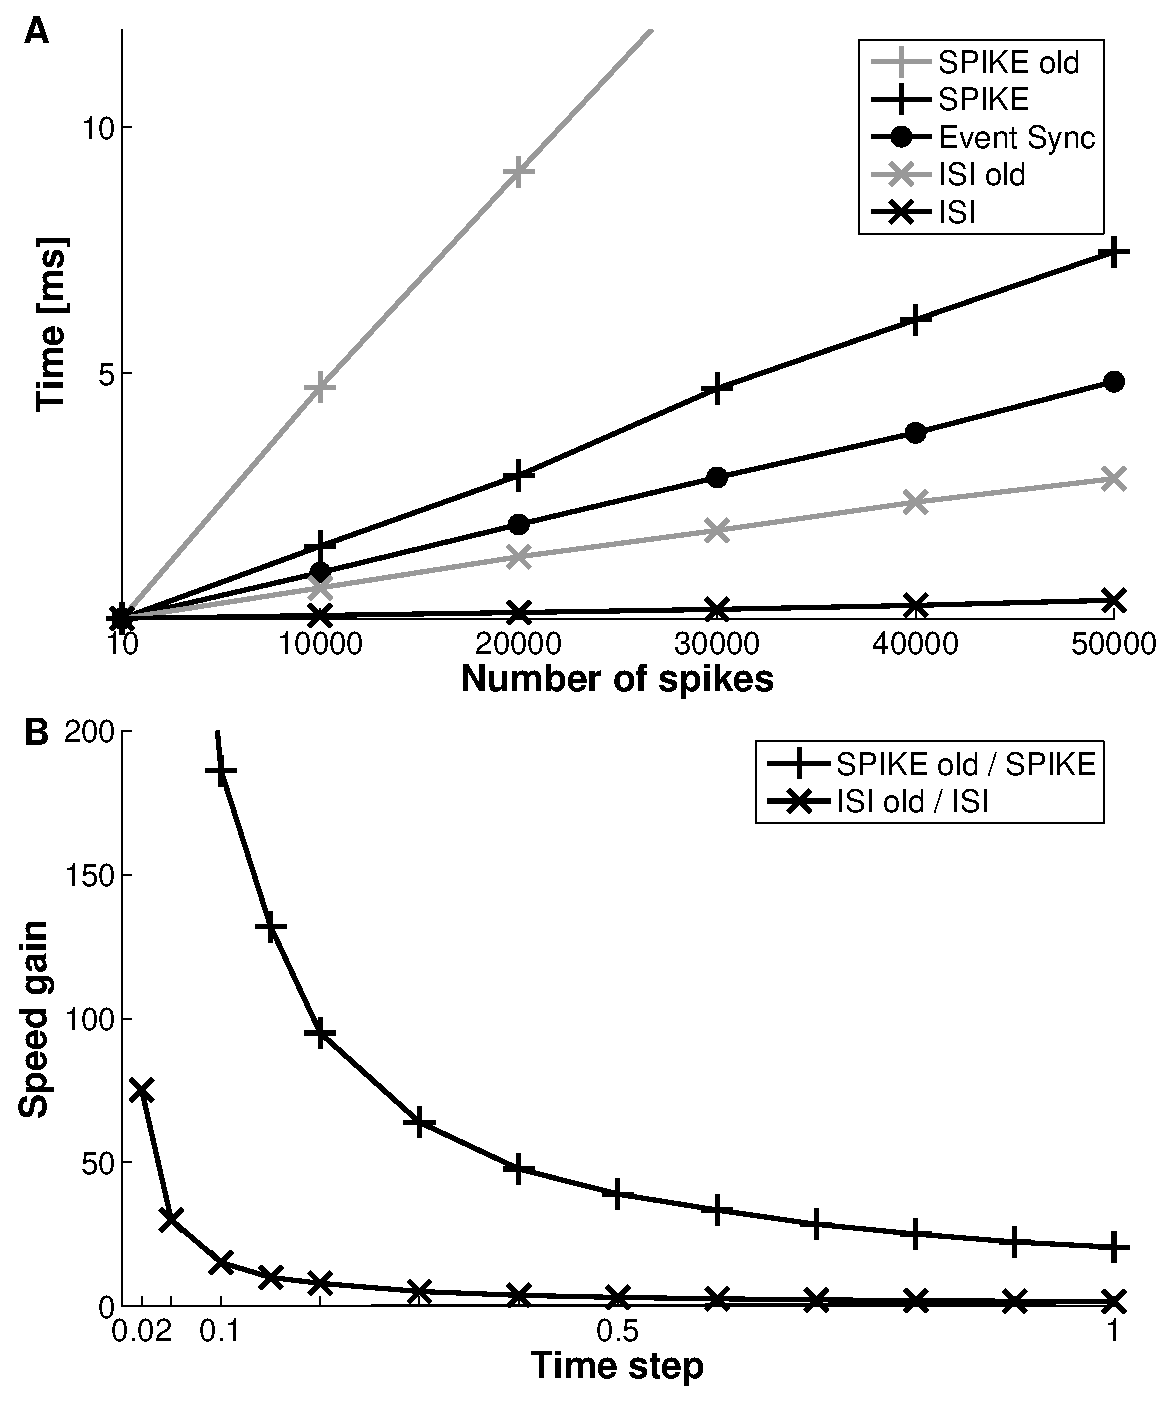
\includegraphics[width=85mm]{Performance_Comparison.eps}
    \caption{\abb\label{fig:Fig5-Performance-Comparison} Performance comparison.   A. Time needed for computing the ISI-distance, the SPIKE-distance, and event synchronization as a function of the number of spikes in each of the two spike trains. For the ISI- and the SPIKE-distance we show the performance improvement from the old (dissimilarity profiles are equidistantly sampled with a sampling interval of $1$ ms) to the new algorithms (optimal spike-dependent sampling). Among the three measures included in SPIKY, event synchronization ranks in between the slower SPIKE-distance and the faster ISI-distance.   B. Dependence of the performance gain between old and new implementation on the sampling interval used for the old implementations. XXXXX Better plot gain factor. This would avoid the two constant lines. XXXXX}
\end{figure}
%
% #########################################################################################
% #########################################################################################
% ############################## Figure: Performance Comparison ###########################
% #########################################################################################
% #########################################################################################




%
% *************************************************************************************
% *************************************************************************************
% ************************************** Section: Discussion **************************
% *************************************************************************************
% *************************************************************************************
%
\section{\label{s:Discussion} Discussion}

\subsection{\label{ss:Summary} Summary}

In this paper we present the graphical user interface SPIKY which facilitates the application of methods of spike train analysis to both simulated and real datasets. Apart from the standard Peri-Stimulus Time Histogram, SPIKY contains three parameter-free and time-resolved measures (see Section \ref{s:Information-reduction}). These measures are complementary to each other since each one addresses a different specific aspect of spike train similarity. While the ISI-distance quantifies local dissimilarities based on covariances of the neurons’ firing rate profiles, both the SPIKE-distance and event synchronization capture the relative timing of spikes. However, whereas the SPIKE-distance weights and normalizes the differences between nearest neighbor spikes, event synchronization acts as a binary coincidence detector, i.e. there is a cutoff at the (adaptive or fixed) time lag relative to which two neighboring spikes are either considered coincident or not and all detailed information both within or outside this coincidence window is discarded.

All of these measures yield instantaneous values for each pair of spike trains, and thus there are many different possible representations of the results (see Section \ref{s:Information-reduction}). Often the most informative representation might depend on the amount and type of spike train data and SPIKY can be used to reveal it via some explorative and interactive analysis. SPIKY also allows to alter a given dataset before or after the actual analysis, e.g., to interactively select subintervals or spike train subsets, to define time markers and spike train separators, and to divide the dataset into different spike train groups. 

In addition to the main GUI designed for the detailed analysis of one dataset, the SPIKY-package also includes two complementary programs. While `SPIKY\_loop' aims at the collective analysis of large numbers of datasets, `SPIKY\_loop\_surro' allows the estimation of significance levels. In all of these programs we use MEX-files, i.e. C-based Matlab executables for the more time-consuming parts and we exploit the piecewise linearity of the dissimilarity profiles, thereby guaranteeing high computation speed and memory efficiency.


\subsection{\label{ss:Limitations} Limitations and caveats}

The calculation of the SPIKE-distance consists of three steps: First for each spike the distance to the nearest spike in all the other spike trains is calculated. Successively, for each time instant and each pair of spike trains, the distances of the four corner spikes are first locally weighted and then normalized. These latter steps involve matrices of the order `number of interspike intervals in the pooled spike train' $\times$ `number of spike train pairs', which for very long datasets with many spike trains can lead to memory problems. The solution to this problem is to make the calculation sequential, i.e., to cut the recording interval into smaller segments, and to perform the averaging over all pairs of spike trains for each segment separately. In the end the dissimilarity profiles for the different segments (already averaged over pairs of spike trains) are concatenated, and its temporal average yields the distance value for the whole recording interval. During this sequential calculation SPIKY uses a waitbar (which displays the \% completed) to continuously inform the user about the progress.

One should be aware that all of these measures are based on some explicit notion of localness and simultaneousness 
and thus they all can be fooled by phase lags, no matter whether these are caused by internal delay loops in one spike train or by a common driver that forces the two time series with different delays. Therefore, any such phase lags should be removed by suitably shifting the time series in a preprocessing step.



\subsection{\label{ss:Outlook} Outlook}

This manuscript is concerned with a new program primarily designed to analyze neuronal spike trains. But in principle it is also applicable to any other kind of discrete data which comes in the form of sequences of time stamps (such as times of bouncing basketballs and coded parent and child acts during children's tantrums just to mention two examples which we already dealt with). Furthermore, in \citet{Kreuz13} we already applied the SPIKE-distance not only to discrete data but also to an example of continuous data (modified EEG). We plan to include this possibility in SPIKY; in principle the only preprocessing step missing is the transformation of the continuous data to discrete data via some kind of spike / event detection.

One of the measures included in SPIKY is the realtime SPIKE-distance. The present algorithm calculates the realtime values by making use of past information only but it does so in a speed-optimized and parallelized manner which would not be compatible with an actual realtime-implementation. However, such a realtime-implementation should actually be simpler and less problematic even for large numbers of neurons since the only information that would have to be stored at each time instant are the time stamps of the latest spikes of each spike train and their nearest neighbors in the other spike trains.

We chose to write SPIKY in Matlab due to its popularity in the neuroscience community, ease of use, and the engaging visualization capabilities of its GUI design. Because of its high level parallelization, Matlab provides a powerful tool for processing vectorized data, but it also includes a well-developed MEX-interface for integrating C functions for performance enhancements. C functions do not only lead to an increase in performance, they can also easily be incorporated into other programming platforms. Indeed, we are about to export at least some of its functionality into an open-source environment (Github-repository) which could for example be based on Python code within a C++ core. XXXXX Check with Mario, start Github-repo now and put link here to get more people on board XXXXX

Another potential direction would be the extension of the methods used here from the quantification of synchrony within one population of two or more neurons to the quantification of synchrony between two (or more) neuronal populations. Similar extensions have been done for two other spike train distances \citep{Aronov03, Houghton08} but both of these methods are not time-resolved and depend on not one but two parameters. So one particular challenge for our methods could be to try to maintain the high temporal resolution of the original methods and to make the new methods parameter-free.

Note that there are many open questions regarding neuronal synchrony. Among these questions are its role in dynamical diseases like epilepsy and its relevance for neural coding. While a thorough discussion of these issues is beyond the scope of this paper, we argue that SPIKY should be a very useful tool for investigation. If epileptic seizures and/or time-dependent stimulations lead to changes in spike train synchrony or spike train clustering, SPIKY should be able to detect them.

%A comprehensive comparison of all proposed methods, done by \cite{Rusu14}, already indicates that the speed of computing distances is converging towards the realtime application. Reaching memory efficiency and solving temporal resolution, would add up to a useful tool to analyze huge amount of data. 



\vspace{1cm}

\begin{thanks}
\section{\label{s:Acknowledgement} \textbf{Acknowledgements}}

NB and TK acknowledge funding support from the European Commission through the Marie Curie Initial Training 	Network `Neural Engineering Transformative Technologies (NETT)', project 289146. TK also acknowledges the Italian Ministry of Foreign Affairs regarding the activity of the Joint Italian-Israeli Laboratory on Neuroscience.

TK thanks Marcus Kaiser for hosting him at the University of Newcastle, UK.
     
We thank Ralph Andrzejak, Emily Caporello, Daniel Chicharro, Tim Gentner, Conor Houghton, Jutta Kretzberg, Stefano Luccioli, Florian Mormann, Mario Mulansky, Leon Paz, Friederice Pirschel, Andreea Sburlea, Alessandro Torcini, Jonathan Victor, and Sid Visser for useful discussions.

We also thank Thomas Alderson, Black Square, Mayte Bonilla Quintana, Hamid Charkhkar, Didier Desaintjan, Mario DiPoppa, Mahboubeh Etemadi, Marion Najac, Matthew Phillips, Eugenio Piasini, Robert Rein, Rodrigo Salazar, Michael Schaub, Eitan Schechtman, Matthew Williams, Yunguo Yu for advice and user feedback.

Finally, we thank Conor Houghton, Mario Mulansky, and Andreea Sburlea for carefully reading the manuscript. XXXXX Check for completeness in the end XXXXX
\end{thanks}


\begin{thebibliography}{25}

\bibitem[{Aronov(2003)}]{Aronov03}
Aronov D, Reich DS, Mechler F, Victor JD. Neural coding of spatial phase in V1 of the macaque monkey. J Neurophysiol, 2003;89:3304-27.

\bibitem[{Bower et al.(2012)}]{Bower12}
Bower MR, Stead M, Meyer FB, Marsh WR, Worrell GA. Spatiotemporal neuronal correlates of seizure generation in focal epilepsy. Epilepsia, 2012;53:807-16.

\bibitem[{{Di Poppa} and Gutkin(2013)}]{DiPoppa13}
{DiPoppa} M, Gutkin BS. Correlations in background activity control persistent state stability and allow execution of working memory tasks. Front Comp Neurosci, 2013;7:139.

\bibitem[{Gruen(2009)}]{Gruen09}
Gr{\"u}n S. Data-Driven Significance Estimation for Precise Spike Correlation. J Neurophysiol, 2009;101:1126-40.

\bibitem[{Hochberg et al.(2006)}]{Hochberg06}
Hochberg LR, Serruya MD, Friehs GM, Mukand JA, Saleh M, Caplan AH, Branner A, Chen D, Penn RD, Donoghue JP. Neuronal ensemble control of prosthetic devices by a human with tetraplegia. Nature, 2006;442:164-71.

\bibitem[{Houghton and Sen(2008)}]{Houghton08}
Houghton C, Sen K. A new multineuron spike train metric. Neural Comput, 2008;20:1495-511.

\bibitem[{Kass et al.(2005)}]{Kass05}
Kass RS, Ventura V, Brown EN. Statistical issues in the Analysis of Neuronal Data. J Neurophysiol, 2005;94:8-25.

\bibitem[{Kreuz et al.(2007)}]{Kreuz07c}
Kreuz T, Haas JS, Morelli A, Abarbanel HDI, Politi A. Measuring spike train synchrony. J Neurosci Methods, 2007;165:151-61.

\bibitem[{Kreuz et al.(2009)}]{Kreuz09}
Kreuz T, Chicharro D, Andrzejak RG, Haas JS, Abarbanel HDI. Measuring multiple spike train synchrony. J Neurosci Methods, 2009;183:287-99.

\bibitem[{Kreuz et al.(2011)}]{Kreuz11}
Kreuz T, Chicharro D, Greschner M, Andrzejak RG. Time-resolved and time-scale adaptive measures of spike train synchrony. J Neurosci Methods, 2011;195:92-106.

\bibitem[{Kreuz(2011)}]{Kreuz11b}
Kreuz T. Measures of spike train synchrony. Scholarpedia, 2011;6:11934.

\bibitem[{Kreuz(2012)}]{Kreuz12}
Kreuz T. SPIKE-distance. Scholarpedia, 2012;7:30652.

\bibitem[{Kreuz et al.(2013)}]{Kreuz13}
Kreuz T, Chicharro D, Houghton C, Andrzejak RG, Mormann F. Monitoring spike train synchrony. J Neurophysiol, 2013;109:1457.

\bibitem[{Kumar et al.(2010)}]{Kumar10}
Kumar A, Rotter S, Aertsen A. Spiking activity propagation in neuronal networks: reconciling different perspectives on neural coding. Nature Rev Neurosci, 2010;11:615-27.

\bibitem[{Louis et al.(2010)}]{Louis10}
Louis S, Gerstein GL, Gr{\"u}n S, Diesmann M. Surrogate spike train generation through dithering in operational time. Front Comp Neurosci, 2010;4:127.

\bibitem[{Mainen and Sejnowski(1995)}]{Mainen95}
Mainen Z, Sejnowski TJ. Reliability of spike timing in neocortical neurons. Science 1995;268:1503-6.

\bibitem[{Miller and Wilson(2008)}]{Miller08}
Miller EK, Wilson MA. All My Circuits: Using Multiple Electrodes to Understand Functioning Neural Networks. Neuron, 2008;60:483-8.

\bibitem[{Mormann et~al.(2007)}]{Mormann07}
Mormann F, Andrzejak RG, Elger CE, Lehnertz K. Seizure prediction: the long and winding road. Brain, 2007;130:314-33.

\bibitem[{Nirenberg and Victor(2007)}]{Nirenberg07}
Nirenberg S, Victor JD. Analyzing the activity of large populations of neurons: how tractable is the problem? Curr Opin Neurobiol 2007;17:397-400.

\bibitem[{Papoutsi et~al.(2013)}]{Papoutsi13}
Papoutsi A, Sidiropoulou K, Cutsuridis V, Poirazi P. Induction and modulation of persistent activity in a layer v pfc microcircuit model. Front Neural Circuits 2013;7:161.

\bibitem[{Pikovsky et~al.(2001)}]{Pikovsky01}
Pikovsky AS, Rosenblum MG, Kurths J. Synchronization. A universal concept in nonlinear sciences. Cambridge Univ. Press, Cambridge, UK 2001.

\bibitem[{Quian Quiroga} et~al.(2002)]{QuianQuiroga02b}
{Quian Quiroga} R, Kreuz T, Grassberger P. Event synchronization: \textsc{A} simple and fast method to measure synchronicity and time delay patterns. Phys Rev E 2002;66:041904.

\bibitem[{Quian Quiroga} and Panzeri(2013)]{QuianQuiroga13}
{Quian Quiroga} R, Panzeri S (Eds.). Principles of neural coding. CRC Taylor and Francis, Boca Raton, FL, USA 2013.

\bibitem[{Ross(1997)}]{Ross97}
Ross SM. Introduction to Probability Models. Sixth edition. Academic Press, New York, USA 1997.

\bibitem[{Rusu and Florian(2014)}]{Rusu14}
Rusu CV, RV Florian. A new class of metrics for spike trains. Neural Computation, 2014;26:306-48.

\bibitem[{Sacr\'{e} and Sepulchre(2014)}]{Sacre14}
Sacr\'{e} P, Sepulchre R. Sensitivity analysis of oscillator models in the space of phase-response curves: Oscillators as open systems. Control Systems, IEEE 2014;34:50–74.

\bibitem[{Sanchez(2008)}]{Sanchez08}
Sanchez JC, Principe JC, Nishida T, Bashirullah R, Harris JG, Fortes JAB. Technology and Signal Processing for Brain-Machine Interfaces. IEEE Signal Processing, 2008;25:29-40.

\bibitem[{Shlens et al.(2008)}]{Shlens08}
Shlens J, Rieke F, Chichilnisky EJ. Synchronized firing in the retina. Curr Opin Neurobiol, 2008;18:396-402.

\bibitem[{Thibeault et al.(2014)}]{Thibeault14}
Thibeault CM, {O'Brien} MJ, Srinivasa N. Analyzing large-scale spiking neural data with HRLAnalysis. Front. Neuroinform., 2014;8:17.

\bibitem[{Tiesinga et al.(2008)}]{Tiesinga08}
Tiesinga PHE, Fellous JM, Sejnowski TJ. Regulation of spike timing in visual cortical circuits. Nature Reviews Neuroscience 2008;9:97-107.

\bibitem[{Truccolo et al.(2011)}]{Truccolo11}
Truccolo W, Donoghue JP, Hochberg LR, Eskandar EN, Madsen JR, Anderson WS, Brown EN, Halgren E, Cash SS. Single-neuron dynamics in human focal epilepsy. Nature Neurosci, 2011;14:635-41.

\bibitem[{Victor(2005)}]{Victor05}
Victor JD. Spike train metrics. Current Opinion in Neurobiology 2005;15:585-592.

\end{thebibliography}

\bibliographystyle{elsart-harv}



%\bibliography{Kreuz_Bibliography}

%\bibliographystyle{jabbrv_plain}
%\bibliographystyle{jneurophysiol}
%\bibliographystyle{plainnat}

\end{document}
